\section{Test}

\subsection{Specifica dei test}

Per garantire la qualità del prodotto, \textit{Three Way Milkshake} adotta il \gls{vmodel}\textsubscript{G} per verificare tramite test ogni passo della produzione software.\\Qui vedremo un immagine rappresentativa del \gls{vmodel}\textsubscript{G} (o V-Model), quest'ultimo si puo' schematizzare posizionando il tempo nell'asse delle ascisse e il livello di astrazione nell'asse delle ordinate.\\Il modello idealmente si divide in 2 rami.\\Il ramo sinistro contiene le fasi di progettazione e ideazione; il ramo destro contiene le fasi di testing e integrazione.
\begin{figure}[h!]
	\centering
	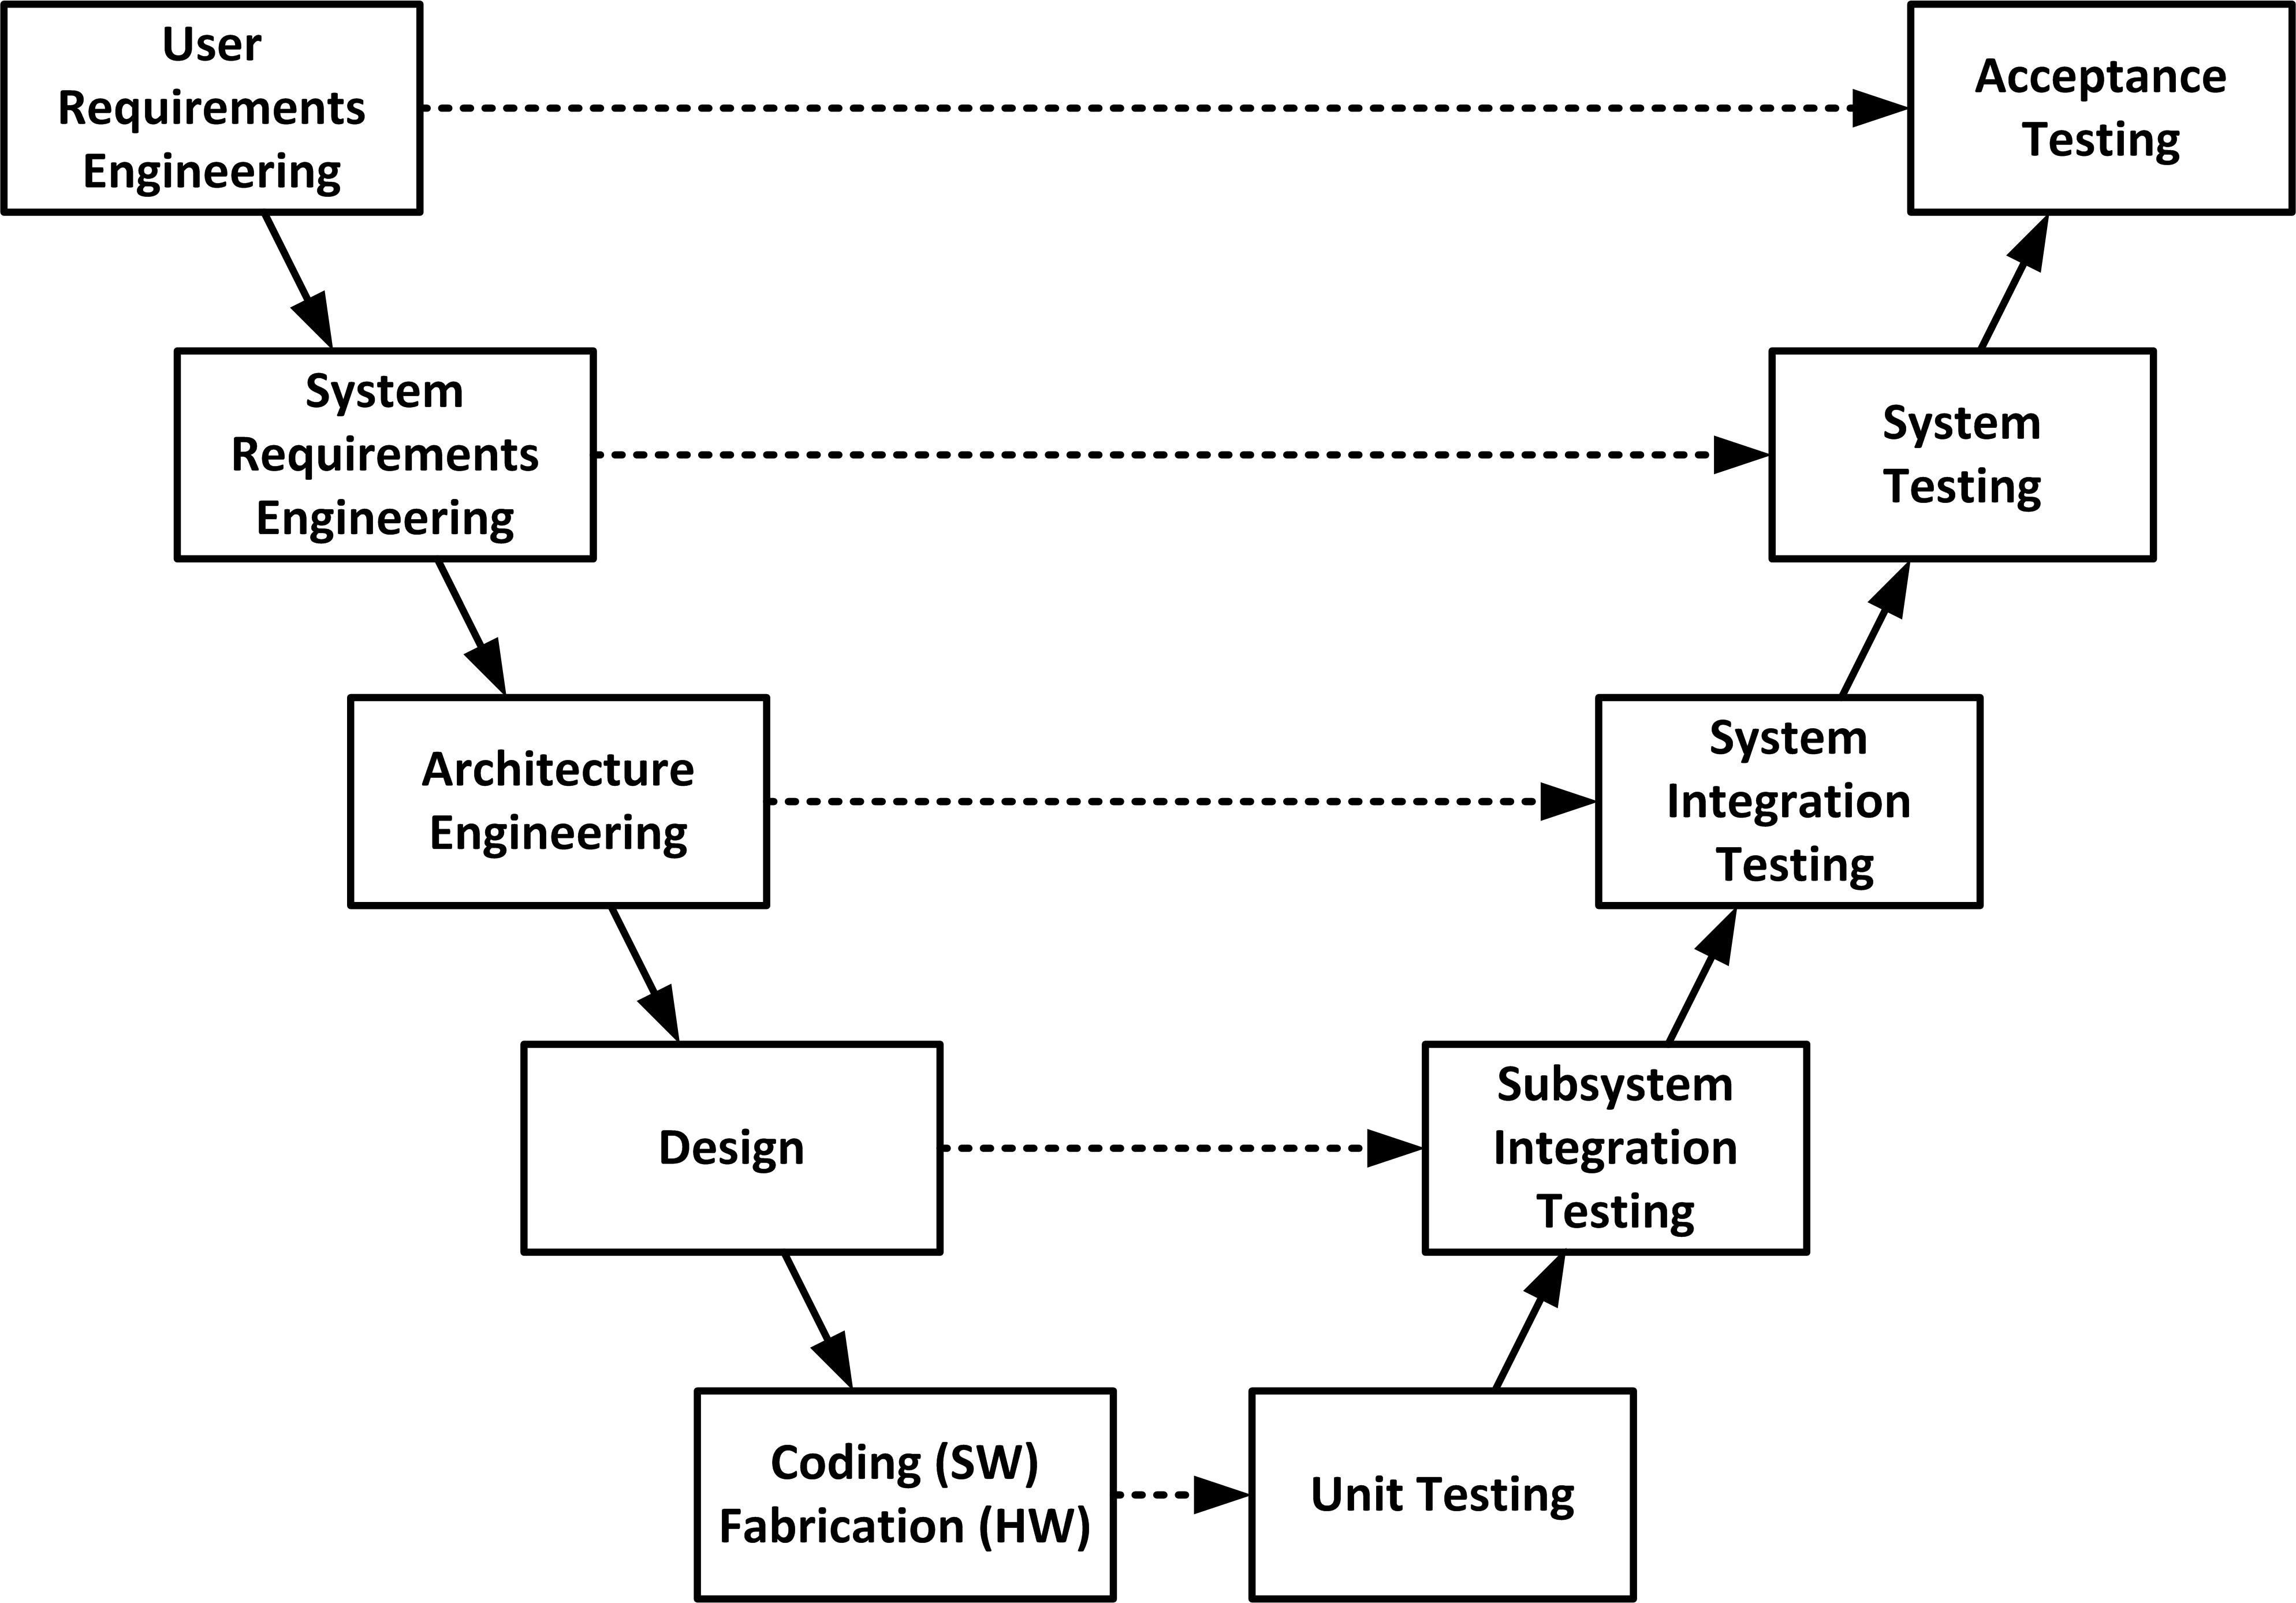
\includegraphics[scale=0.6]{res/images/v_model.jpg}
	\caption{Figura esplicativa del \gls{vmodel}\textsubscript{G}}
\end{figure}

Per definire lo stato dei test viene utilizzato un valore da 0 a 2:
\begin{itemize}
	\item \textbf{0:} - Il test non è stato implementato;
	\item \textbf{1:} - Il test è stato implementato, ma fallisce;
	\item \textbf{2:} - Il test è stato implementato ed è stato superato.
\end{itemize}
Vi sono quattro tipi di test:
\begin{itemize}
	\item Test di Accettazione;
	\item Test di Sistema;
	\item Test di Integrazione;
	\item Test di Unità.
\end{itemize}
\subsection{Test di Accettazione}
I Test di Accettazione verificano che il software nel suo complesso soddisfi i criteri di accettazione decisi con il cliente.\\I test di accettazione verranno indicati nel seguente modo:\\
\begin{center}
	TA[Importanza][Tipo][Codice]\\
\end{center}
ove:
\begin{itemize}
	\item \textbf{Importanza:} indica l'importanza del requisito tra i seguenti livelli d'importanza:
		\begin{itemize}
			\item \textbf{O} per i requisiti obbligatori;
			\item \textbf{D} per i requisiti desiderabili;
			\item \textbf{F} per i requisiti facoltativi.
		\end{itemize}
	\item \textbf{Tipo:} indica il tipo dei requisiti tra i seguenti tipi:
		\begin{itemize}
			\item \textbf{F} per i requisiti funzionali;
			\item \textbf{V} per i requisiti di vincolo;
			\item \textbf{Q} per i requisiti di qualità;
			\item \textbf{P} per i requisiti prestazionali.
		\end{itemize}
	\item \textbf{Codice:} rappresenta il codice identificativo crescente del componente da verificare.
\end{itemize}
%tabella
\subsection{Test di Sistema}
I Test di Sistema verificano la conformità dell'intero sistema con i requisiti specificati.\\I Test di Sistema verranno sviluppati quando verrà raggiunta la fase appropriata, secondo il \gls{vmodel}\textsubscript{G}.

\subsection{Test di Integrazione}
I Test di Integrazione verificano l'integrazione di più componenti software o hardware.\\I Test di Integrazione verranno sviluppati quando verrà raggiunta la fase appropriata, secondo il \gls{vmodel}\textsubscript{G}.

\subsection{Test di Unità}
I Test di Unità verificano le parti atomiche del software (per esempio funzioni o procedure). Vengono utilizzati per assicurarsi che la logica interna del codice sia rispettata.\\I Test di Unità verranno sviluppati quando verrà raggiunta la fase appropriata, secondo il \gls{vmodel}\textsubscript{G}.

\subsection{Resoconto attività di verifica}
\subsubsection{Esiti dell'indice di Gulpease}
%tabella